\chapter{Survival and re-entry dynamics}
\label{app:survival}

The selection mechanism of Section~\ref{sec:growing-degree-size} can be measured directly rather
than inferred from the survivor-size relation. Figure~\ref{fig:survival-degree} shows the
conditional survival probability for ten independent power-law-$2.5$ economies of $N = 10000$,
with $C=N/40=250$, at the operating point of the main text. A firm counts as a survivor when its
share remains above $10^{-6}$ throughout the late window $t\in[180,240]$. We calculate a rate in
each degree bin within each economy and then average the ten rates with equal weight. The bands
are $95\%$ $t$ intervals across economies, not intervals from a pooled supergraph.

Survival falls sharply with degree: the rate is $0.159\pm0.049$ in the lowest resolved bin
($k\approx75$), $0.044\pm0.015$ at $k\approx352$, and $0.014\pm0.008$ at
$k\approx985$; no survivor is observed above $k\approx2760$. This is the direct selection step
behind the degree--size relation: connectivity broadens the disorder field but competition removes
the typical high-degree firm. The graph construction itself has no sampled degrees below $k=58$,
so the figure makes no claim about a distinct low-degree network ensemble.

\begin{figure}[htbp]
    \centering
    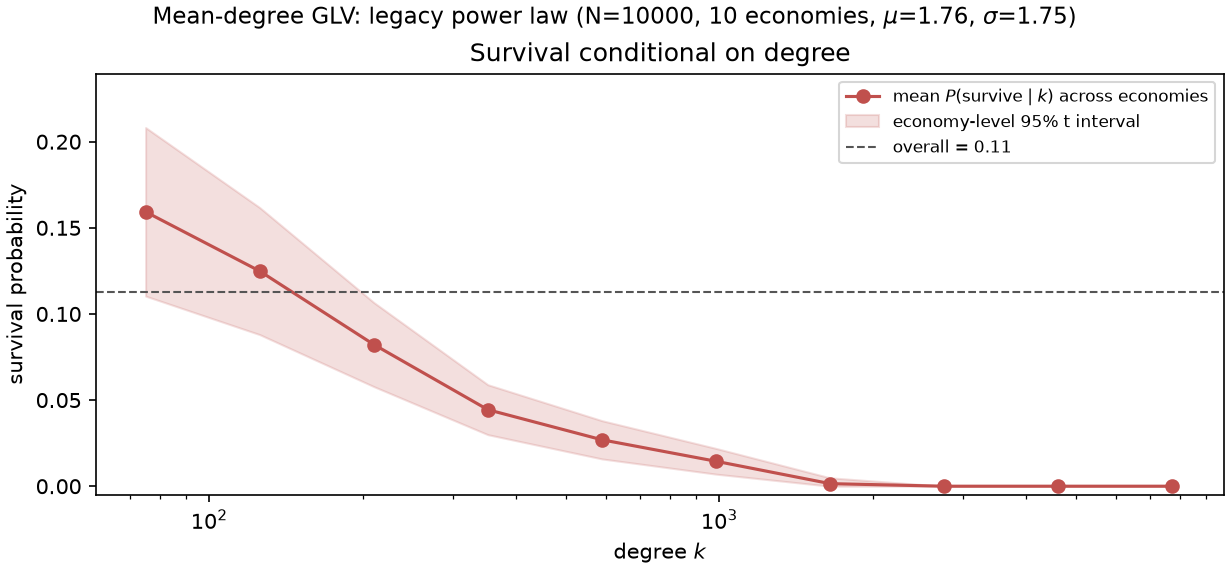
\includegraphics[width=\linewidth]{survival_by_degree.png}
    \caption{Survival conditional on degree in the thesis mean-degree power-law ensemble
    ($N=10000$, $C=250$, ten economies, $\mu=1.76$, $\sigma=1.75$). Each point is the unweighted
    mean of the within-economy survival probabilities; shading is the $95\%$ interval across
    economies. A firm is counted as surviving only if its share stays above $10^{-6}$ throughout
    $t\in[180,240]$. The probability falls steadily across the resolved support, directly exposing
    the competitive selection of hubs.}
    \label{fig:survival-degree}
\end{figure}

Crossing the threshold is not an absorbing extinction event. In the same ten trajectories we
classify a re-entry only when a firm is active, drops below the threshold, and later returns above
it; a first activation does not count. Although
only $11.3\%$ of firms remain above the threshold throughout the whole window, $87.5\%$ are active
at some point. Among firms that exit at least once, $85.4\%$ re-enter before the window ends
(Figure~\ref{fig:reentry-degree}). The re-entry probability conditional on an exit is $0.87$ in
the lowest resolved degree bin and remains $0.77$ at $k\approx985$, falling only in the
sparsely populated extreme tail. The low persistent-survival probability therefore records
turnover around the threshold rather than irreversible firm loss. Immigration continually reseeds
low shares, while the fluctuating interaction field can return a firm to the active set.

\begin{figure}[htbp]
    \centering
    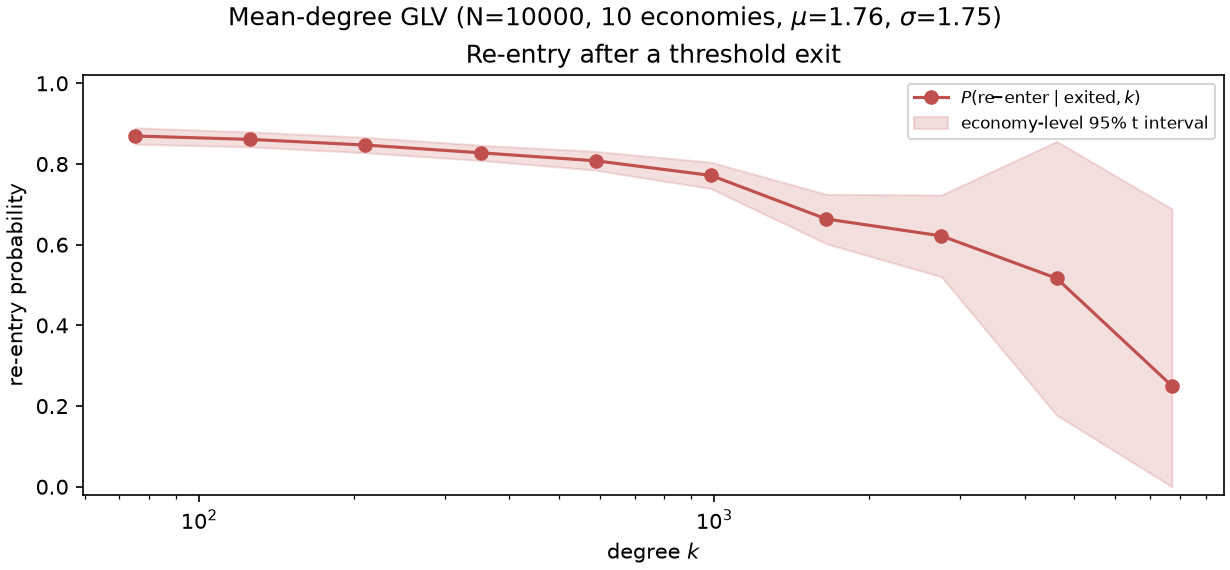
\includegraphics[width=\linewidth]{reentry_by_degree.png}
    \caption{Re-entry after a threshold exit in the thesis mean-degree power-law ensemble
    ($N=10000$, $C=250$, ten economies, $\mu=1.76$, $\sigma=1.75$). A re-entry requires an
    active--inactive--active sequence within $t\in[180,240]$; first activation is excluded.
    Each point is the unweighted mean of the within-economy probability
    $P(\mathrm{re\!\!\! - \! enter}\mid\mathrm{exited},k)$, with $95\%$ intervals across
    economies. The high re-entry rate makes explicit that threshold exits are churn, not
    absorbing extinctions.}
    \label{fig:reentry-degree}
\end{figure}
